\textbf{Цель работы:} при помощи модели абсолютно чёрного тела проведение измерения температуры оптическим пирометром с исчезающей нитью и термопарой; определение постоянных Планка и Стефана-Больцмана.

\textbf{В работе используются:} оптический пирометр, модель абсолютно чёрного тела (АЧТ), вольфрамовая лампа, неоновая лампа, блок питания, цифровые вольтметры.
                    
\section{Теоретическое введение}

    Для измерения температуры разогретых тел, удалённых от наблюдателя, применяют методы оптической пирометрии, основанные на использовании зависимости испускательной способности исследуемого тела от температуры. Различают три температуры, функционально связанные с истинной термодинамической температурой и излучательной способностью тела: радиационную $T_{rad}$, цветовую $T_{col}$ и яркостную $T_{br}$.

    В работе измеряется яркостная температура -- температура абсолютно чёрного тела, при которой его спектральная испускательная способность равна спектральной испускательной способности исследуемого тела при той же длине волны.
    Измерение яркостной температуры раскалённого тела производится при помощи оптического пирометра с исчезающей нитью, основанного на визуальном сравнении яркости раскалённой нити с яркостью изображения исследуемого тела. Равенство видимых яркостей, наблюдаемых через монохроматический светофильтр ($\lambda = 650$ нм), фиксируется по исчезновению изображения нити на фоне раскаленного тела.
    Яркостный метод измерения температуры основан, в соответствии с формулой Планка, на зависимости испускательной способности абсолютно чёрного тела от температуры и длины волны.

    Шкалу прибора, измеряющего ток через нить, предварительно градуируют по абсолютно черному телу, термодинамическую температуру которого измеряют с помощью термопары. Если тело, температуру которого определяют, излучает как абсолютно черное тело, то, мы тем самым можем с помощью пирометра найти его температуру. Если же тело излучает иначе, то определенное значение температуры является яркостной температурой. Яркостная температура тела всегда
    ниже его термодинамической температуры.

    Среди нечерных тел выделяются так называемые серые тела, для которых характер распределения излучения совершенно подобен спектру абсолютно черного тела, но излучение ослаблено по сравнению с ним в $\varepsilon_T$ раз для любой длины волны при данной температуре тела $T$. Если предположить, что тело излучает как серое тело, то выражения для энергии излучения можно записать как
    \begin{equation*}
        W = \varepsilon_T S \sigma T^4,
    \end{equation*}
    с учётом того, что температура тело намного больше температуры окружающей среды и мощностью внешних потерь можно пренебречь.


\section{Экспериментальная установка}

    Экспериментальная установка состоит из оптического пирометра 9, модели абсолютно черного тела (АЧТ), трех исследуемых
    образцов \\ ($18, 19, 20$), блока питания (1) и цифровых вольтметров В7-22А и В7-38.

    Оптический пирометр представляет собой зрительную трубу, внутри которой имеется накаливаемая нить, расположенная в плоскости
    изображения исследуемого раскаленного тела, а также темно-красный светофильтр ($\lambda = 650$ нм). Через окуляр одновременно наблюдается
    изображение исследуемого тела и раскаленной нити.

    Модель АЧТ представляет собой керамическую трубку диаметром
    $3$ мм и длиной $50$ мм, закрытую с одного конца и окруженную для
    теплоизоляции внешним кожухом. Нагрев трубки осуществляется намотанной на ней нихромовой спиралью, питаемой от источника тока.
    Полость трубки и особенно ее дно излучают практически как абсолютно черное тело. Температура модели АЧТ измеряется хромельалюмелевой термопарой, один спай которой вмонтирован в дно трубки, а другой находится при комнатной температуре на клемме цифрового вольтметра В7-38, измеряющего ЭДС термопары.

    В работе исследуются три образца. Один образец выполнен в виде керамической трубки с набором колец из различных материалов,
    нагреваемой изнутри нихромовой спиралью. Другой исследуемый образец -- вольфрамовая нить электрической
    лампочки. Она питается от источника 1, когда переключатель 6 находится в положении 3. Сила тока через вольфрамовую нить измеряется
    с помощью прибора В7-22А (15). Падение напряжения на самой нити измеряется непосредственно вольтметром В7-22А (16). Таким образом,
    зная показания обоих приборов, можно определить мощность, потребляемую нитью лампочки.

    \begin{figure}[h!]
        \centering
        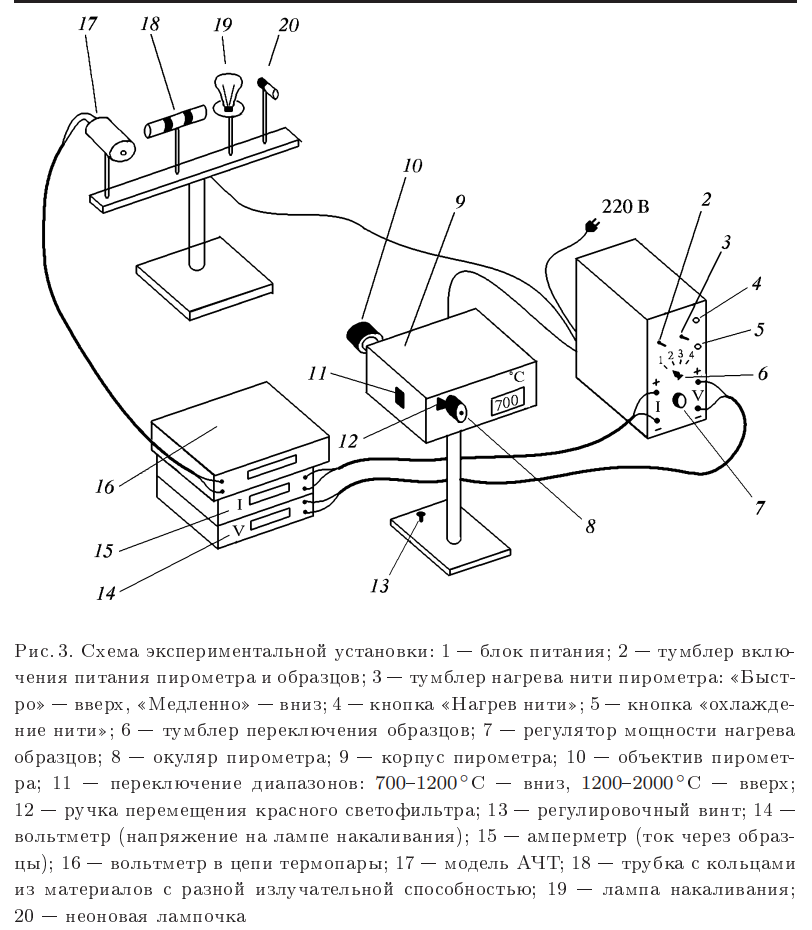
\includegraphics[width = 13 cm]{images/exp_pic}
        \label{exp_pic}
    \end{figure}
    

\section{Ход работы}

\subsection{Изучение работы оптического пирометра}

    Цель пункта: помощью пирометра измеряется температура модели АЧТ и проводится сравнение её значения со значением температуры, измеренной при помощи термопарного термометра.

\begin{enumerate}
    \item Настроим пирометр, прогреем его нить. Прогреем модель АЧТ.
    \item Введём красный светофильтр пирометра. Изменяя ток через нить пирометра, добьёмся исчезновения нити на фоне изображения раскалённой поверхности дна АЧТ.

    \begin{table}[h]
        \centering
        \begin{center}
            \caption{Сравнение температур АЧТ, выдаваемое пирометром и измеренное термпопарой}
        \end{center}
        \begin{tabular}{|l|l|l|l|l|l|l|}
        \hline
        $T$, $^\circ C$ (убывание)          & 936  & 936 & 931 & 934 & $\langle T \rangle $, $^\circ C$ & $934 \pm 5$  \\ \cline{1-5} \cline{7-7} 
        $T$, $^\circ C$ (возрастание)       & 928  & 927 & 931 & 933 & $\langle T \rangle $, $^\circ C$ & $930 \pm 5$ \\ \hline
        $V$, мВ                            & \multicolumn{4}{l|}{37,41} & $T_{\text{термопара}}$, $^\circ C$              & $938 \pm 2$        \\ \hline
        \end{tabular}
        \label{table:comparison}
    \end{table}

\end{enumerate}

    Из таблицы следует, что пирометр проградуирован по АЧТ точно в пределах погрешностей измерений.

\subsection{Измерение яркостной температуры накалённых тел}

    При нагревании керамической трубки с помощтю пирометра зафиксировано, что различные кольца обладают различными яркостными температурами вследствие различяи спектральных светимостей. Яркостные температуры тел измерить не удалось из-за того, что свечения колец оказалось достаточно слабым (невозможно определить, одинаковы ли яркости нити и кольца).

\subsection{Проверка закона Стефана-Больцмана}

    Нагреем лампу накаливания ло тёмно-красного свечения, а затем будем увеличивать её температуру, снимая значения силы тока и напряжения на лампе. Измеренная яркостная температура преобразуется в термодинамическую температуру с помощью графика завивимости $T(T_{\text{ярк}})$. 

    \begin{figure}[h!]
        \centering
        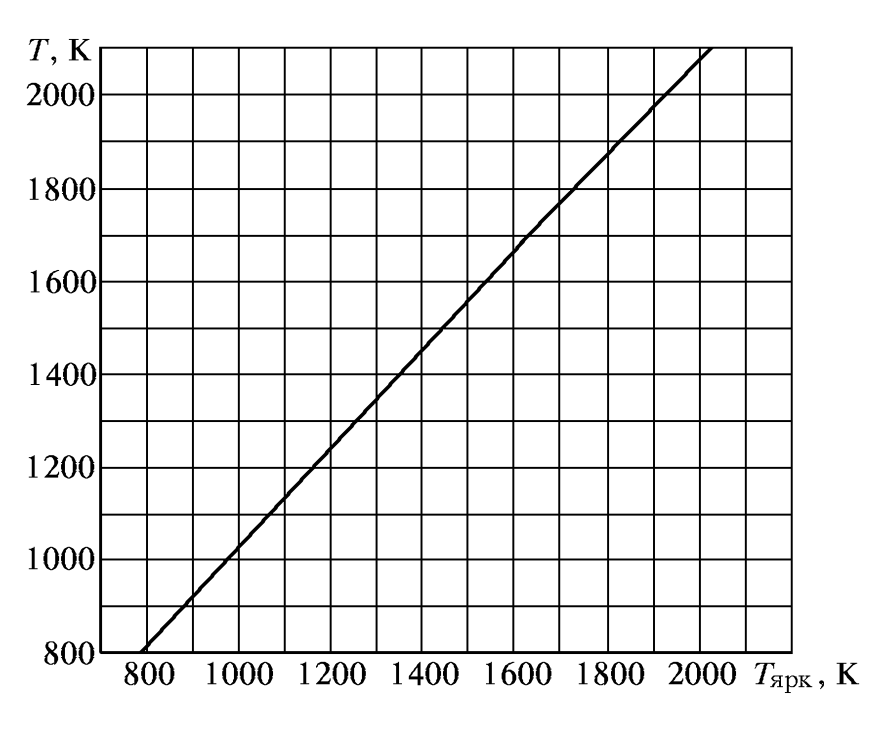
\includegraphics[width = 11 cm]{images/wolfram_tempr}
        \caption{График зависимости $T(T_{\text{ярк}})$ для лампы накаливания (вольфрам)}
        \label{}
    \end{figure}

    Закон Стефана-Больцмана в случае вольфрамовой лампы накаливания для проверки имеет вид
    \begin{equation}
        W = \varepsilon_T S \sigma T^n \Rightarrow \ln W = \ln (\varepsilon_T S \sigma) + n \ln T,
    \end{equation}
    или
    \begin{equation}
        \ln W - \ln (\varepsilon_T S \sigma) = n \ln T,
    \end{equation}
    где $\varepsilon_T = \varepsilon_T (T)$, зависимость представлена в виде таблицы для различных температур вольфрама, а $S = \; 5 \text{см}^2$ -- площадь поверхностей нитей накаливания.

    \begin{figure}[h!]
        \centering
        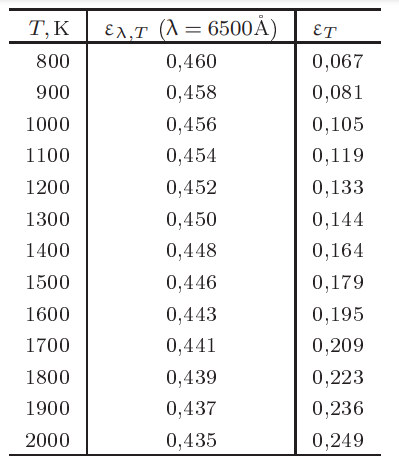
\includegraphics[width = 6.5 cm]{images/wolfram_coef}
        \caption{Таблица коэффициентов $\varepsilon_T$ для вольфрама}
        \label{}
    \end{figure}

    Построим таблицу измеренных значений.

    \begin{table}[h!]
        \centering
        \begin{tabular}{|c|c|c|c|c|}
        \hline
        $T_{\text{ярк}}$, $^\circ C$ & $T$, K  & $V$, мВ & $I$, А & $W$, мВт \\ \hline
        857.00              & 1135.18 & 58.14   & 1.077  & 62.62  \\ \hline
        942.00              & 1227.91 & 79.2    & 1.277  & 101.14 \\ \hline
        1024.00             & 1317.36 & 105.65  & 1.491  & 157.52 \\ \hline
        1082.00             & 1380.63 & 129.84  & 1.662  & 215.79 \\ \hline
        808.00              & 1081.73 & 46.14   & 0.952  & 43.93  \\ \hline
        839.00              & 1115.55 & 52.05   & 1.016  & 52.88  \\ \hline
        893.00              & 1174.45 & 66.43   & 1.159  & 76.99  \\ \hline
        919.00              & 1202.82 & 69.23   & 1.202  & 83.21  \\ \hline
        996.00              & 1286.82 & 93.78   & 1.396  & 130.92 \\ \hline
        1059.00             & 1355.54 & 128.85  & 1.663  & 214.28 \\ \hline
        \end{tabular}
        \caption{Измеренные значения для лампы накаливания (вольфрам)}
    \end{table}
    
    \begin{figure}[h!]
        \centering
        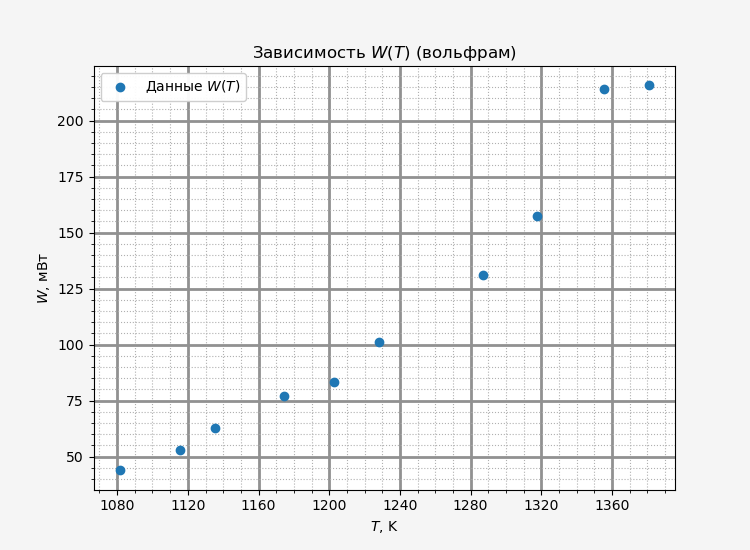
\includegraphics[width = 13 cm]{images/WT}
        \caption{График зависимости $W(T)$}
        \label{}
    \end{figure}

    \begin{figure}[h!]
        \centering
        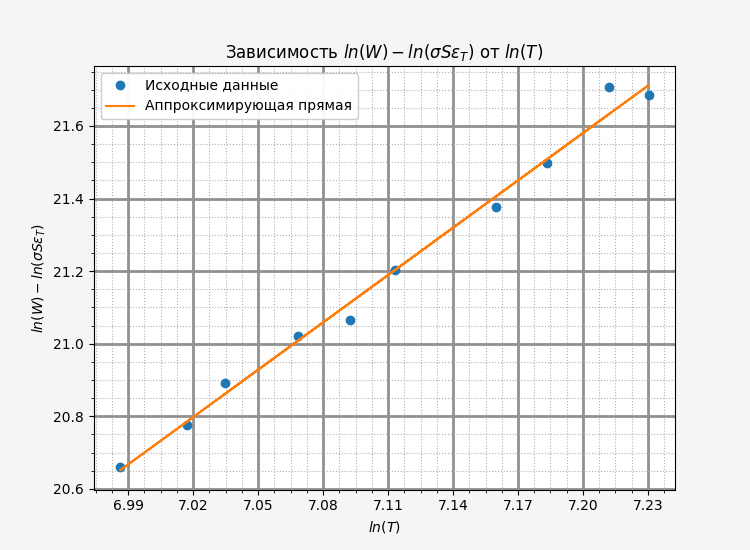
\includegraphics[width = 13 cm]{images/WT_ln}
        \caption{График зависимости $W(T)$ в логарифмических осях}
        \label{}
    \end{figure}
    
    С помощью МНК измерим коэффициент из логарифмического графика $W(T)$:
    \begin{equation*}
        n = 4.34, \Delta n = 0.29, R^2 = 0.991
    \end{equation*}
    Полученное значение в рамках погрешностей сходится с теоретическим значением, равным 4 (закон Стефана-Больцмана).

    С учётом того, что для лампы накаливания $S = 5 \; \text{см}^2$, посчитаем для 3 различных температур ($T = 1174.45 \; K, T = 1380.63 \; K, T = 1081.73 K$) в рамках всего температурного диапазона значения постоянной Стефана-Больцмана (значения $\varepsilon_T$ посчитаны из таблицы):

    $$ \sigma_1 = (5.31 \pm 0.21) \cdot 10^{-9} \; \text{Вт} \cdot \text{м}^2 \cdot \text{К}^{-4} $$
    $$ \sigma_2 = (6.33 \pm 0.17) \cdot 10^{-9} \; \text{Вт} \cdot \text{м}^2 \cdot \text{К}^{-4} $$
    $$ \sigma_3 = (7.24 \pm 0.15) \cdot 10^{-9} \; \text{Вт} \cdot \text{м}^2 \cdot \text{К}^{-4} $$
    
    Полученные значения на порядок отличаются от теоретического значения постоянной Стефана-Больцмана.

\subsection{Измерение яркостной температуры неоновой лампочки}

    Термодинамическая температура неоновой лампочки примерно равна комнатной и не соответствует её яркостной температуре ($T_{\text{якр}} = \approx 828 ^\circ C$). Дело в том, что неоновая лампочка в принципе не является моделью абсолютно чёрного или серого тела, и её излучение носит совершенно другую природу (переход электронов между энергетическими уровнями). Неоновая лампа имеет похожую спектральную светимость при заданной длине волны $\lambda = 650$ нм, хотя её температура совсем не соответствует яркостной.


\section{Заключение}

    В результате работы проверена градуировка пирометра по АЧТ -- при значении, измеренном термопарой $(938 \pm 2) ^\circ C$, получены значения термодинамической температуры при убывании яркостной температуры во время измерений $(934 \pm 5) ^\circ C$ и при возрастании $(930 \pm 5) ^\circ C$. То есть значения, измеренные по пирометру, в рамках погрешностей совпадают со значением, измеренным термопарой.

    Для двух колец, изготовленных из различных материалов, зафиксировано различие яркостных температур при $\lambda = 650$ нм при одинаковых термодинамических температурах, т.к. различные материалы могут иметь различные зависимости спектральной светимости от длины волны.

    Подтверждена температурная зависимость закона Стефана-Больцмана для лампы накаливания (вольфрам) с результатами степени
    \begin{equation*}
        W \propto T^n, n = 4.34, \Delta n = 0.29, n_{th} = 4.
    \end{equation*}

    Во всём диапазоне измерений найдены постоянные Стефана-Больцмана для 3 различных температур $T = 1174.45 \; K, T = 1380.63 \; K, T = 1081.73 K$:
    $$ \sigma_1 = (5.31 \pm 0.21) \cdot 10^{-9} \; \text{Вт} \cdot \text{м}^2 \cdot \text{К}^{-4} $$
    $$ \sigma_2 = (6.33 \pm 0.17) \cdot 10^{-9} \; \text{Вт} \cdot \text{м}^2 \cdot \text{К}^{-4} $$
    $$ \sigma_3 = (7.24 \pm 0.15) \cdot 10^{-9} \; \text{Вт} \cdot \text{м}^2 \cdot \text{К}^{-4} $$
    Полученные значения отличаются на порядок от теоретического $\sigma = 5.67 \cdot 10^{-8} \; \text{Вт} \cdot \text{м}^2 \cdot \text{К}^{-4}$. Причины расхождения возможны из-за неверно заданной площади поверхности нитей лампы накаливания $S = 5 \; \text{см}^2$ (которая не влияет на поиск температурной зависимости $W(T)$), также возможны расхождения из-за того, что в рассчётах не учитываются потери на рассеивание тепла в окружающую среду (воздух).

    Для неоновой лампы измереноа яркостная температура $T_{\text{якр}} \approx 828 ^\circ C$ и проверено, что её термодинамическая темпаратура отличается от яркостной и примерно равна комнатной.


